\documentclass[a4 paper]{article}
% Set target color model to RGB
\usepackage[inner=2.0cm,outer=2.0cm,top=2.5cm,bottom=2.5cm]{geometry}
\usepackage{setspace}
\usepackage[rgb]{xcolor}
\usepackage{verbatim}
\usepackage{subcaption}
\usepackage{amsgen,amsmath,amstext,amsbsy,amsopn,tikz,amssymb,tkz-linknodes}
\usepackage{fancyhdr}
\usepackage[colorlinks=true, urlcolor=blue,  linkcolor=blue, citecolor=blue]{hyperref}
\usepackage[colorinlistoftodos]{todonotes}
\usepackage{rotating}
%\usetikzlibrary{through,backgrounds}
\hypersetup{%
pdfauthor={Ashudeep Singh},%
pdftitle={Assignment 4},%
pdfkeywords={Tikz,latex,bootstrap,uncertaintes},%
pdfcreator={PDFLaTeX},%
pdfproducer={PDFLaTeX},%
}
%\usetikzlibrary{shadows}
% \usepackage[francais]{babel}
\usepackage{booktabs}
\newcommand{\ra}[1]{\renewcommand{\arraystretch}{#1}}

\newtheorem{thm}{Theorem}[section]
\newtheorem{prop}[thm]{Proposition}
\newtheorem{lem}[thm]{Lemma}
\newtheorem{cor}[thm]{Corollary}
\newtheorem{defn}[thm]{Definition}
\newtheorem{rem}[thm]{Remark}
\numberwithin{equation}{section}

\newcommand{\homework}[6]{
   \pagestyle{myheadings}
   \thispagestyle{plain}
   \newpage
   \setcounter{page}{1}
   \noindent
   \begin{center}
   \framebox{
      \vbox{\vspace{2mm}
    \hbox to 6.28in { {\bf COMP 3005:~Database Management Systems \hfill {\small (#2)}} }
       \vspace{6mm}
       \hbox to 6.28in { {\Large \hfill #1  \hfill} }
       \vspace{6mm}
       \hbox to 6.28in { {\it Instructor: {\rm #3} \hfill Name: {\rm #5}, ID: {\rm #6}} }
       %\hbox to 6.28in { {\it TA: #4  \hfill #6}}
      \vspace{2mm}}
   }
   \end{center}
   \markboth{#5 -- #1}{#5 -- #1}
   \vspace*{4mm}
}

\newcommand{\problem}[2]{~\\\fbox{\textbf{Q #1}}\hfill (#2 points)\newline\newline}
\newcommand{\subproblem}[1]{~\newline\textbf{(#1)}}
\newcommand{\D}{\mathcal{D}}
\newcommand{\Hy}{\mathcal{H}}
\newcommand{\VS}{\textrm{VS}}
\newcommand{\solution}{~\newline\textbf{\textit{(Solution)}} }

\newcommand{\bbF}{\mathbb{F}}
\newcommand{\bbX}{\mathbb{X}}
\newcommand{\bI}{\mathbf{I}}
\newcommand{\bX}{\mathbf{X}}
\newcommand{\bY}{\mathbf{Y}}
\newcommand{\bepsilon}{\boldsymbol{\epsilon}}
\newcommand{\balpha}{\boldsymbol{\alpha}}
\newcommand{\bbeta}{\boldsymbol{\beta}}
\newcommand{\0}{\mathbf{0}}



\begin{document}
\homework{Assignment \#4}{Due: Friday Apr. 3, 2020 (11:59 PM)}{Ahmed El-Roby}{}{}{}
\textbf{Instructions}: Read all the instructions below carefully before you start working on the assignment, and before you make a submission.
\begin{itemize}
    \item The accepted formats for your submission are: pdf and docx. More details below. 
    \item If you use the tex file, make sure you edit line 28 to add your name and ID. Only write your solution and do not change anything else in the tex file. If you do, you will be penalized.
    \item Late submissions are allowed for 24 hours after the deadline above with a penalty of 10\% of the total grade of the assignment. Submissions after more than 24 are not allowed.
\end{itemize}

\problem{1:}{3}
In variable-length record representation, the record starts with offset and length pairs of variable-size attributes, followed by fixed-size attributes, then the null bitmap, and finally the variable-size attributes. How can we improve this representation if our application is expected to store tables with large number of attributes, most of which are nulls?



\problem{2:}{4}
Consider the following arrangement for four disks, where $B_{i}$ is a data block, and $P_{i}$ is the parity block for the 4 data blocks that precedes it. What problem will this arrangement cause?

{\centering 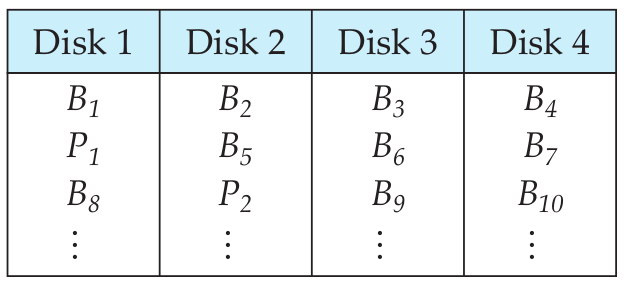
\includegraphics[width=\textwidth/2]{figure1.png}}





\problem{3:}{9}
Consider the following file organization using free list.

{\centering 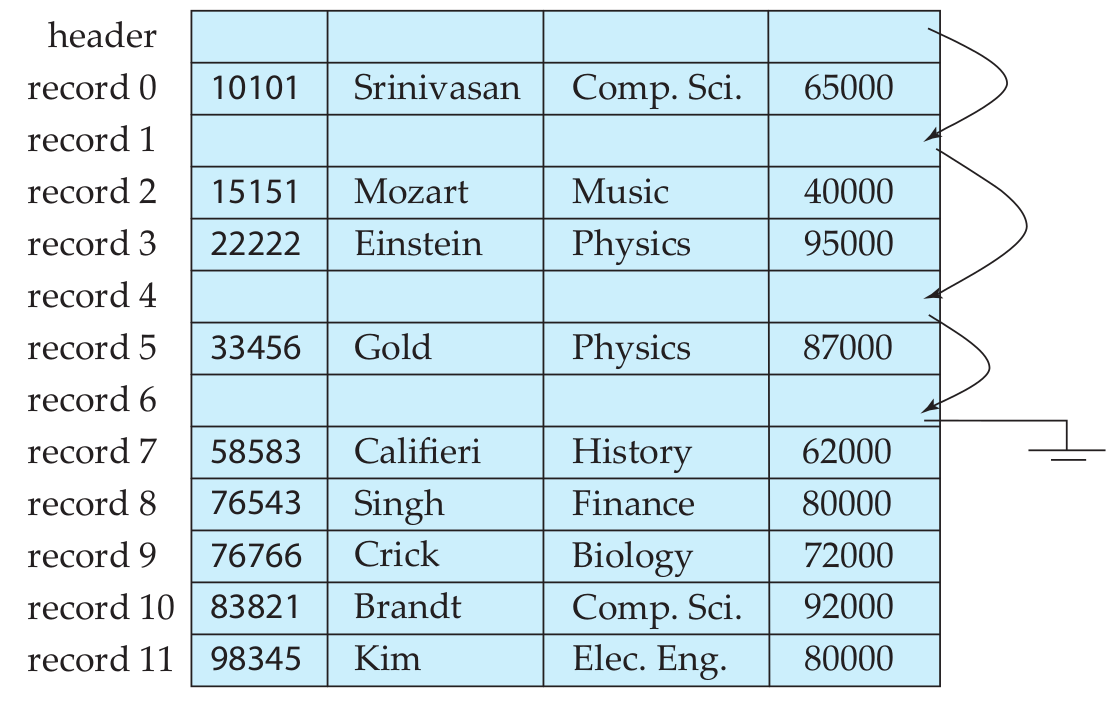
\includegraphics[width=\textwidth/2]{figure2.png}}

\noindent Show the structure of the file after each of the following operations (they follow each other):

\subproblem{a} Delete record 9.\indent (2 marks)




\subproblem{b} Insert (20000, Jamie, Physics, 100000).\indent (3 marks)





\problem{4:}{12}
Construct a $B^{+}$-tree for the following set of key values: (2, 3, 5, 7, 11, 17, 19, 23, 29, 31). The tree is initially empty and values are added one value at a time in ascending order. Consider the following values of $n$:
\subproblem{a} $n = 4$.\indent \indent (4 points)
\subproblem{b} $n = 6$.\indent \indent (4 points)
\subproblem{c} $n = 8$.\indent \indent (4 points)






\problem{3:}{8}
Consider the following $B^{+}$-tree with $n = 4$:
\begin{figure}[h]
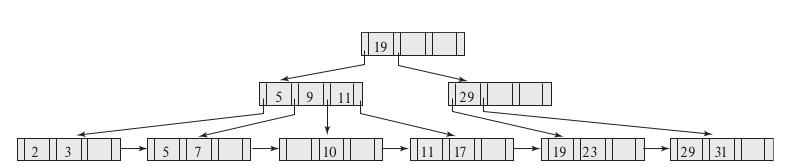
\includegraphics[height=2in, width=6in]{tree-delete.png}
\end{figure}

\subproblem{a} Delete 23.\indent \indent (4 points)



\subproblem{b} Delete 19.\indent \indent (4 points)



\problem{4:}{4}
Consider the following $B^{+}$-tree with $n = 6$:
\begin{figure}[h]
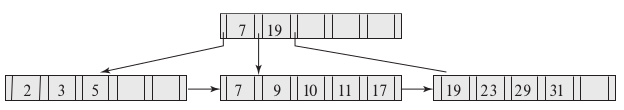
\includegraphics[height=1in, width=5in]{tree-insert.png}
\end{figure}
Insert 8 into this tree.


\end{document}

